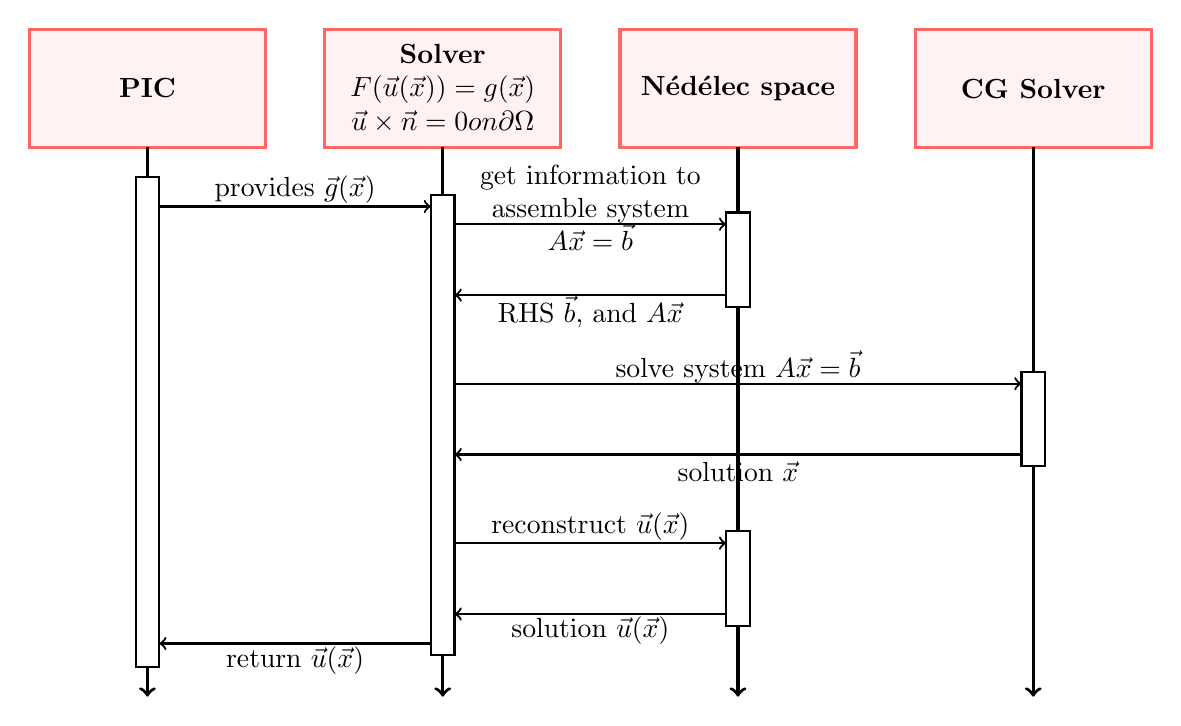
\begin{tikzpicture}[scale=1.5,every text node part/.style={align=center}]

    % Head
    \filldraw[draw=red!60, fill=red!5, very thick] (0,0) rectangle (2,-1) node[pos=0.5]{\textbf{PIC}};
    \filldraw[draw=red!60, fill=red!5, very thick] (2.5,0) rectangle (4.5,-1) node[pos=0.5]{\textbf{Solver} \\ $F(\vec{u}(\vec{x})) = g(\vec{x})$ \\ $\vec{u}\times \vec{n} = 0 \text{ on } \partial \Omega$};
    \filldraw[draw=red!60, fill=red!5, very thick] (5,0) rectangle (7,-1) node[pos=0.5]{\textbf{Nédélec space}};
    \filldraw[draw=red!60, fill=red!5, very thick] (7.5,0) rectangle (9.5,-1) node[pos=0.5]{\textbf{CG Solver}};
    
    % Tails
    \draw[very thick, ->] (1,-1) -- (1,-5.65);
    \draw[very thick, ->] (3.5,-1) -- (3.5,-5.65);
    \draw[very thick, ->] (6,-1) -- (6,-5.65);
    \draw[very thick, ->] (8.5,-1) -- (8.5,-5.65);


    % Things
    \filldraw[draw=black, fill=white, thick] (0.9,-1.25) rectangle (1.1,-5.4);
    \draw[->, thick] (1.1,-1.5) -- (3.4,-1.5) node[pos=0.5,yshift=6] {provides \(\vec{g}(\vec{x})\)};
    \filldraw[draw=black, fill=white, thick] (3.4,-1.4) rectangle (3.6,-5.3);
    \draw[->, thick] (3.6,-1.65) -- (5.9,-1.65) node[pos=0.5,yshift=6] {get information to\\assemble system\\\(A\vec x = \vec{b}\)};
    \filldraw[draw=black, fill=white, thick] (5.9,-1.55) rectangle (6.1,-2.35);
    \draw[->, thick] (5.9,-2.25) -- (3.6,-2.25) node[pos=0.5,yshift=-6] {RHS \(\vec{b}\), and \(A\vec{x}\)};
    \draw[->, thick] (3.6,-3) -- (8.4,-3) node[pos=0.5,yshift=6] {solve system \(A\vec{x} = \vec{b}\)};
    \filldraw[draw=black, fill=white, thick] (8.4,-2.9) rectangle (8.6,-3.7);
    \draw[->, thick] (8.4,-3.6) -- (3.6,-3.6) node[pos=0.5,yshift=-6] {solution \(\vec{x}\)};
    \draw[->, thick] (3.6,-4.35) -- (5.9,-4.35) node[pos=0.5,yshift=6] {reconstruct \(\vec{u}(\vec{x})\)};
    \filldraw[draw=black, fill=white, thick] (5.9,-4.25) rectangle (6.1,-5.05);
    \draw[->, thick] (5.9,-4.95) -- (3.6,-4.95) node[pos=0.5,yshift=-6] {solution \(\vec{u}(\vec{x})\)};
    \draw[->, thick] (3.4,-5.2) -- (1.1,-5.2) node[pos=0.5,yshift=-6] {return \(\vec{u}(\vec{x})\)};


\end{tikzpicture}